\chapter{Planning and Methodology}
\label{cap:plan}

\section{Feasibility Study}

Before initiating any project, it is of utmost importance to conduct a
comprehensive analysis of relevant factors to gauge the likelihood of
accomplishing successful outcomes. While estimating the complexity associated
with developing, deploying, and maintaining machine learning (ML) systems is
indeed a challenging task, it is essential to recognize that this project
encompasses not only the research aspect but also significant software and
infrastructure development. \\

This project requires a careful balancing act, as it involves dedicating
efforts to both the research and practical implementation aspects. The
development of robust software and infrastructure is crucial to support the
successful integration of the deep learning models and ensure their efficient
deployment and maintenance. This integration can be intricate and demanding, as
it requires a deep understanding of both the ML algorithms and the software
engineering principles. \\

In light of these additional dimensions, the study not only aims to evaluate
the feasibility of utilizing deep learning techniques but also strives to
address the complexities inherent in developing a well-rounded solution.
Furthermore, the evaluation will consider the available data and resources to
assess the potential of achieving satisfactory results.

\section{Technical Study}

The journey begins with research, a dynamic element that evolves and gains
strength through continuous investigation. While it is impossible to guarantee
the achievement of all objectives, the way we see it, there are three
fundamental pillars that must be addressed in advance. \\

\subsection{Defining the Use Case}

Academic researchers may find satisfaction in uncovering effective solutions
that contribute to publications and secure additional funding. Yet, this thesis
aims to ensure the successful implementation of a Computer-Aided Diagnosis
(CAD) infrastructure specifically designed for classifying melanoma, with the
intention of deploying it in real-world scenarios we needed to look further
than just the pure research. \\

\subsection{Equipment and Technical Knowledge}

Equipment and technical knowledge are interdependent and collectively
contribute to the success of a machine learning project. \\

In a deep learning project, both the availability of suitable equipment and
technical knowledge are essential. The correct equipment, including high
performance computing resources and data collection devices, facilitates
efficient data handling, prepossessing, model training, and deployment.
Simultaneously, technical knowledge plays a vital role in effectively
leveraging the available equipment. Understanding diverse machine learning
algorithms and methodologies assists in selecting the most appropriate
approaches for the problem at hand. Additionally, it is crucial to acknowledge
the knowledge required to create other services that accompany the project. \\

\subsection{Importance of the Dataset}

The success of a project like this one depends not only on the quantity but
also on the quality of the data. Data is essential for any deep learning model
to learn effectively. Therefore, it is vital to invest time in acquiring an
optimal image data-set that possesses sufficient data volume, annotation,
truth, and reusability. \\

For computer-based image recognition and analysis, high-quality data is
necessary. The objective is to gather data from various patient populations to
ensure that the data-set is diverse and accurately represents different disease
states and outcomes. Often, healthcare organizations engage medical experts to
review and label the data to prevent inaccurate labels and ensure the
data-set's significance, as is the case in this project.

\section{Economical Study}

In this section we give you and over-view of the material and human cost to
develop the thesis.

\subsection{Equipment Cost}

Equipment cost pertains to the expenditure incurred on hardware and software
licenses necessary for the project. \\

The hardware and software used in the project are listed in the \textit{Table
\ref{table:equipment_cost}}.

\begin{table}[H]
  \centering
  \begin{tabular}{lccc}
    \toprule
    \textbf{Component} & \textbf{Units} & \textbf{Unit Price} & \textbf{Cost} \\
    \midrule
    Computer & 1 & \$800 & \$800 \\
    Software (Pytorch, Svelte, FastAPI, etc) & 1 & \$0 & \$0 \\
    Tesla T4, 16GB (GPU)* & 1 & \$2000 & \$2000 \\
    Nvidia A100, 80GB (GPU)* & 1 & \$15000 & \$15000 \\
    \bottomrule
  \end{tabular}
  \caption[The Cost of Components.]
  {\textit{The Cost of Components.
  Components marked with (*) were not paid for out of my own pocket; instead, they were borrowed from VICOROB or
  Google Services. Table by Author}}
  {\label{table:equipment_cost}}
\end{table}

\subsection{Human Resources}

In this section, a hypothetical scenario is presented, illustrating multiple
work profiles contributing to the project and the associated costs for each
service. However, it is important to note that in reality, all tasks were
performed by a single individual. \\

For the thesis we would need this roles: \\

\begin{itemize}
  \item \textbf{Data Scientist}

    Data scientists focus on managing and analyzing data throughout the
    project. They acquire relevant datasets, preprocess the data, develop deep
    learning models, train and evaluate models, and deploy them in production
    environments (some cases). \\

    The average hourly wage for a Data Scientist in United States is
    \textbf{\$36} \cite{SalaryDataScientist}. \\

  \item \textbf{Research Scientist}

    Research scientists focus on the exploration and innovation aspects of deep
    learning projects. Their roles typically include, literature review:
    Research scientists survey existing literature, stay updated with the
    latest advancements in deep learning, and identify relevant research papers
    or techniques that can be applied to the project. Innovation and
    Experimentation: They contribute to the development of novel deep learning
    architectures, techniques, or algorithms to address specific project
    challenges or improve model performance. \\

    The average hourly wage for a Computer Research Scientist in United States
    is \textbf{\$121.163} \cite{SalaryResearchScientist}. \\

  \item \textbf{Data Engineer}

    Data engineers are typically in charge of creating the user interface (UI)
    components of the application that interact with the deep learning models.
    But the most important tasks handled by this profile would be data
    pre-processing, API development, and model integration. They would build
    the necessary APIs to communicate with the deep learning models. \\

    The average hourly wage for a Data Engineer in United States is
    \textbf{\$48} \cite{SalaryDataEnginner}. \\

\end{itemize}

The general tasks that each profile should accomplish and the expected time to
being develop as well as the cost of this hours, is given in \textit{Table
\ref{table:human_resources_cost}}.

\newpage

\begin{table}[H]
  \centering
  \begin{tabular}{lcccc}
    \toprule
    \textbf{Task} & \textbf{Profile} & \textbf{Time} & \textbf{Cost} \\
    \midrule
    Definition and boundaries of the project & Research Scientist & 50h & \$6,081.5\\
    Data collecting & Data Engineer & 10h & \$480\\
    Data preprocessing & Data Engineer & 10h & \$480 \\
    Data analysis and visualization & Data Scientist & 30h & \$1,080\\
    Model development & Research Scientist & 60h & \$7,297.8 \\
    Model training & Data Scientist & 80h & \$2,880 \\
    Model optimization & Data Scientist & 120h & \$4,320 \\
    Models reports & Data Scientist & 20h & \$720 \\
    CAD infrastructure & Data Engineer & 220h & \$10,560 \\
    Infrastructure deployment & Data Engineer & 20h & \$960 \\
    Documentation & Research Scientist & 100h & \$12,163 \\
    \midrule
    \textbf{Total} &    &  \textbf{720h} & \textbf{\$47,022.3} \\
    \bottomrule
  \end{tabular}
  \caption[Human Resources Estimated Cost.]
  {\textit{Human Resources Estimated Cost. Table by Author}}
  {\label{table:human_resources_cost}}
\end{table}


\section{Methodology}

The project methodology employed in this endeavor follows a continuous process
that builds upon previous approaches. Additionally, the project incorporates
the concept of utilizing idle time effectively. For instance, during the
training of models, there are periods of idle time, which we exploited by
concurrently working on other tasks related to developing the entire
infrastructure. This approach allows for maximizing productivity throughout the
project. The various stages involved in the methodology are as follows: \\

\begin{enumerate}

  \item Identifying the problem and establishing the research objectives.
  \item Conducting background research by reviewing prior publications addressing similar or related issues.
  \item Choosing the correct programming languages and frameworks.
  \item Study of the characteristics and distribution of the working data-set.
  \item Familiarizing oneself with the tools and frameworks that will be utilized.The term "equipment cost" pertains to the expenditure incurred on hardware and software licenses necessary for this project.
  \item Breaking down the project into smaller tasks.
  \item Selecting a specific task.
  \item Trying to implement the task in a smart manner.
  \item Developing the task.
  \item Make GPU do its job for certain number of epochs (Iddle).

    \begin{itemize}
      \item Choosing or resuming a develop task (API, UI or Virtualization).
      \item Developing process.
        \begin{itemize}
          \item Developing interruption because model is already trained or because early stopped. Go to point 11.
          \item If there are remaining tasks, choose a new develop task.
        \end{itemize}
    \end{itemize}


  \item Evaluating whether the results meet the expectations.

    \begin{itemize}
      \item If the results fall short of expectations, return to step 8.
      \item If the results meet the expectations, proceed to step 12.
    \end{itemize}

  \item Collecting the necessary artifacts and presenting the results in a clear and appealing manner.

  \item Deploy models.

  \item Deploy the CAD system infrastructure.

  \item Write down the report.

\end{enumerate}

\textit{Figure \ref{fig:flux_development}} Illustrates the previous process by making use of a diagram.

\newpage


\begin{figure}[H]
  \centering
  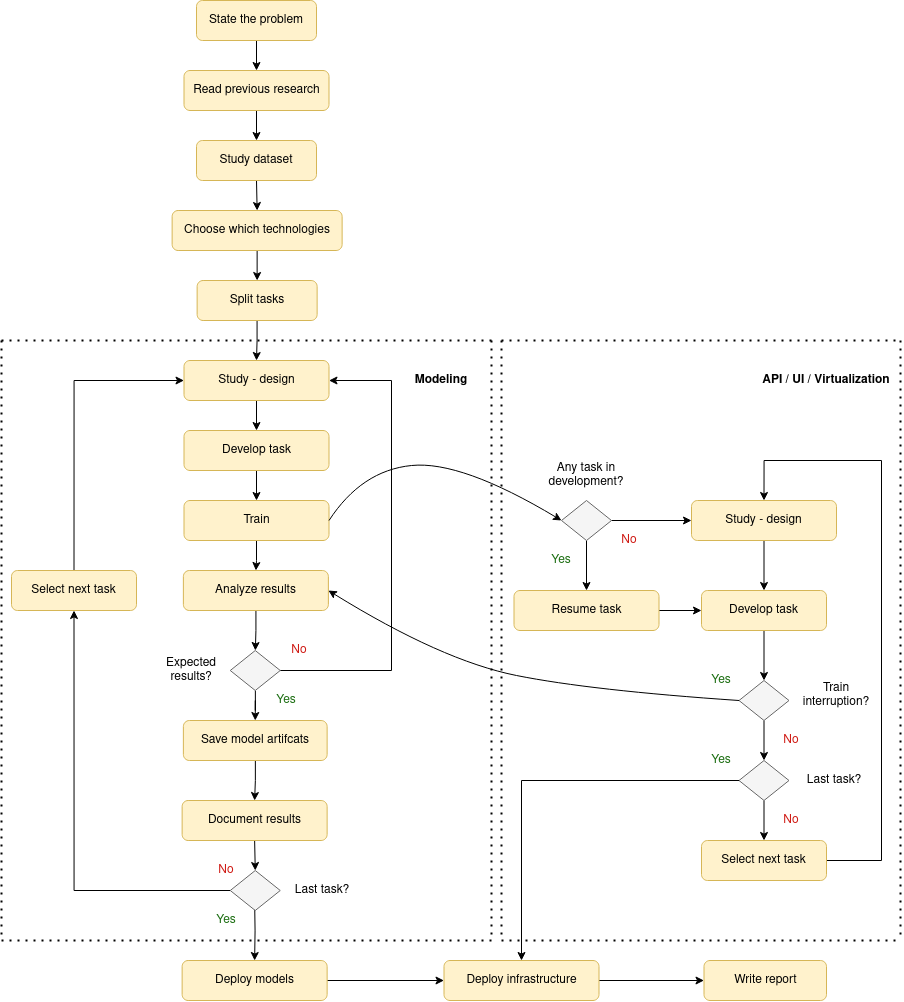
\includegraphics[width=\textwidth]{imatges/planing_and_methodology/EmplyedMethodology.png}
  \caption[Activity Diagram Describing the Methodology.]{\textit{Activity Diagram Describing the Workflow Methodology: Notice that the right workflow is executed every time models are trained and returns to the model evaluation once the models have been trained to analyze results. Illustration by Author}}
  {\label{fig:flux_development}}
\end{figure}


\newpage


\section{Planning}

This thesis was developed under an inter-ship in the Accenture S.L. company,
under the category of Research, innovation, and development. The intern-ship
was thought to conduct the Master thesis at the University of Girona. We also
had the help from VICOROB laboratory which is the Computer Vision and Robotics
Research Group of the University of Girona. This thesis runs under the guidance
of Dr. Rafel Garcia (UdG) and Luis Llopis (Accenture SL) from 1st of December,
2022 to 12th of July of 2023. \\

From now on, we present the outline of the activities entailed in this thesis
and present an approximate scheduler table to visually depict the allocation of
days for their anticipated completion.

\subsection{Tasks}

The task presented here are general, each of this task can be divided in other
multiples tasks.

\begin{itemize}
  \item{\textbf{Defining the Boundaries of the Project}}

    Before commencing the actual work, we spent several days engaging in
    discussions to determine the specific problem we aimed to solve, assess the
    available data-set, and determine the most suitable technologies to
    effectively address the problem. This involved researching available
    melanoma competitions and selecting a technology stack for the project in
    agreement with the advisors.

  \item{\textbf{Setting Up the Environment}}

    The next weeks was mostly devoted to install and make simple test with the
    frameworks selected in the previous step. It resulted in setting up the
    machine with a suitable environment before the development and experimental
    phase. It should be noted that all other tasks were developed with my
    personal computer except the training process that was develop using Google
    Collab service and VICOROB machines.

  \item{\textbf{Study of the Dataset}}

    After setting up the environment, we delved into working with the selected
    database and carefully we examined the distribution of the data-set. It
    became evident that we were dealing with a multi-class unbalanced data-set,
    with certain classes being significantly underrepresented compared to
    others. \\

    Furthermore, we soon realized that due to the substantial size of the
    data-set and the machine learning techniques we wanted to apply, it was not
    feasible to train the model using any of the devices we had at disposal.
    The computational requirements exceeded the capabilities of our available
    resources.

  \item{\textbf{Searching of Existing Literature}}

    Prior to initiating the actual work, a dedicated few weeks were allocated
    to conducting an extensive literature review. This crucial step provided
    valuable insights and a deeper understanding of the proposed research. It
    involved thoroughly reading academic papers and previous theses that
    focused on melanoma detection utilizing convolutional neural networks (CNN)
    or shared a similar research focus.

  \item{\textbf{Acquiring Working Knowledge}}

    Once we had a base knowledge of the problem, we started to follow tutorials
    for each technology that was evolved in the project. \\

    Below is a list of the primary sources we utilized to acquire knowledge
    about various technologies.

    \begin{itemize}
      \item PyTorch: \cite{LearnPyTorch} In this course they teach you the foundations of machine learning and deep learning with PyTorch. The course is video based.

      \item SvelteKit: \cite{LearnSvelteKit} The official SvelteKit documentation.

      \item FastAPI: \cite{LearnFastAPI} The official FastAPI documentation.

      \item Virtualization: To work with virtualization. We made use of two container based tools. Docker \cite{LearnDocker} and Podman \cite{LearnPodman} are the tools used to create the images and container of this project.
    \end{itemize}

  \item{\textbf{Modeling and Development}}

    The development process is comprised of various smaller tasks, as depicted
    in the development flow diagram \textit{Figure \ref{fig:flux_development}}.
    During the modeling stage, numerous models were trained using the available
    data and resources at the time. Additionally, during idle periods of model
    training, we focused on other aspects of the project. This involved
    creating a user interface (UI) specifically designed for professionals to
    interact with, as well as developing an API that is independent of the UI.
    The API facilitates image loading and inference using the selected model.
    Furthermore, extensive testing was conducted to deploy these services and
    configure individual volumes for optimal performance.

  \item{\textbf{Deployment}}

    After developing the CAD infrastructure and uploading the source code to a
    private GitHub repository, and training the models, we proceeded to upload
    the configurations and trained models to a public GitLab repository at
    \url{https://gitlab.com/wilberquito/open.thesis}. They can be easily
    downloaded using Git\footnote{Git is version control software designed by
    Linus Torvalds}. However, it's important to note that deployment may be
    restricted by authentication at the moment of reading this thesis. \\

    The final step of the deployment process involved creating a shell script.
    This script is responsible for downloading the source code from GitHub, as
    well as retrieving the trained models and configurations from GitLab. It
    then utilizes the configuration files specific to each service to create
    the necessary
    images and instantiate the containers accordingly.

  \item{\textbf{Writing the Report}}

    While certain chapters were written throughout the process, the last month
    proved to be crucial for completing the final chapters, expand the chapters
    already written and incorporating any recommended changes suggested by the
    advisors.

\end{itemize}

\newpage

\subsection{Timeline}

\begin{table}[H] \centering
  \begin{tabular}{| l | c | c | c |}
    \hline
    \multicolumn{1}{|c|}{\textbf{Task}} & \multicolumn{1}{c|}{\textbf{Time}} & \multicolumn{1}{c|}{\textbf{Color}} \\
    \hline
    Definition and boundaries of the project & 40h & \cellcolor{red!50} \\
    \hline
    Setting up the environment & 20h & \cellcolor{lime!50} \\
    \hline
    Study of the data-set & 20h & \cellcolor{blue!40} \\
    \hline
    Searching of existing literature & 60h & \cellcolor{teal!50} \\
    \hline
    Acquiring working knowledge & 180h & \cellcolor{amber!30} \\
    \hline
    Modeling and development & 240h & \cellcolor{black!70} \\
    \hline
    Deployment & 40h & \cellcolor{gray!50} \\
    \hline
    Writing the report & 120h & \cellcolor{orange!50} \\
    \hline
    \textbf{Total} & \textbf{720h} & \\
    \hline
  \end{tabular}
  \caption[Estimated Hours per Task.]{\textit{Estimated Hours per Task. Table by Author}}
  {\label{table:timeline_tasks}}
\end{table}

\begin{table}[H]
  \centering
  \label{tab:340W}
  \begin{tabular}{| c | c | c | c |c | c | c |c | c | c |c | c | c |c | }
    \hline
    tasks/weeks & 0 & 3 & 6 & 9 & 12 & 15 & 18 & 21 & 24 & 27 & 30 \\
    \hline
    T1  & \cellcolor{red!50} &   &   &   &   &   &   &   &   &   &     \\
    \hline
    T2  &   & \cellcolor{lime!50}  &  &  &   &   &   &    &  &  &   \\
    \hline
    T3  &  &  & \cellcolor{blue!40} &  &   &   &   &   &  &  & \\
    \hline
    T4  &  &  &  & \cellcolor{teal!50} & \cellcolor{teal!50} &  &  &   &   &   &   \\
    \hline
    T5  &  &  &  &  & \cellcolor{amber!30} & \cellcolor{amber!30} & \cellcolor{amber!30}  & \cellcolor{amber!30} & \cellcolor{amber!30}  &  & \\
    \hline
    T6  &  &  &  &  & \cellcolor{black!70} & \cellcolor{black!70} & \cellcolor{black!70}  & \cellcolor{black!70} & \cellcolor{black!70}  &  \cellcolor{black!70} & \\
    \hline
    T7  &   &  &  &  &  &  &  &   &    & \cellcolor{gray!50} & \\
    \hline
    T8  &   &  &  &  &  & \cellcolor{orange!50}  &  &   &   & \cellcolor{orange!50} & \cellcolor{orange!50} \\
    \hline
  \end{tabular}
  \caption[Estimated Timeline.]
  {\textit{Estimated Timeline.
  All tasks has been scheduled in a timeline that starts from the first week to last the week.
  The time window is three weeks.
  Table by Author}}
\end{table}
